\chapter{Empirical Analysis}
\label{chap:empirical_analysis}

\section{Overview of the Dataset}
\label{subsec:overview_dataset}
This section provides an initial descriptive overview of the aggregated ICIJ dataset, highlighting key structural characteristics that inform the subsequent, more focused and detailed analyses. We begin by examining the geographical concentration of entities, intermediaries, and officers, followed by the degree distribution of intermediaries.

\subsubsection{Concentration of Entities, Intermediaries, and Officers}
\label{subsubsec:concentration_elements}
A striking initial observation from the data is the high degree of geographical concentration in offshore activities across all node types. The complex web of global offshore finance, while spanning over 200 countries and territories in the ICIJ data, appears to be significantly anchored in a relatively small number of key locations. Approximately 98\% of all entities incorporated within the dataset are registered in just 15 jurisdictions. This intense concentration in a few select jurisdictions aligns with literature suggesting that offshore financial centers (OFCs) often specialize in particular 'legal technologies' or cater to specific clienteles, leading to certain jurisdictions becoming dominant hubs for offshore incorporation (Laffitte, 2024).

This pattern of concentration extends to the actors involved. When examining the top 15 countries or jurisdictions associated with each category, we find that around 70\% of entities (by their associated operational countries), 70\% of intermediaries (by their listed country of operation), and 70\% of officers (by their listed country) are concentrated within these leading locations. Figure \ref{fig:preliminary_geography_overview} provides a visual representation of these geographical distributions, illustrating the percentage of entities located in specific jurisdictions, entities active in various countries, intermediaries based in different countries, and officers linked to particular countries. This concentration of intermediaries, for instance, may reflect the clustering of professional services in major global financial centers, as noted by Stausholm and Garcia-Bernardo (2024) - though they concentrate specifically on tax experts - rather than solely in traditional tax havens. 

\begin{figure}[htbp]
    \centering
    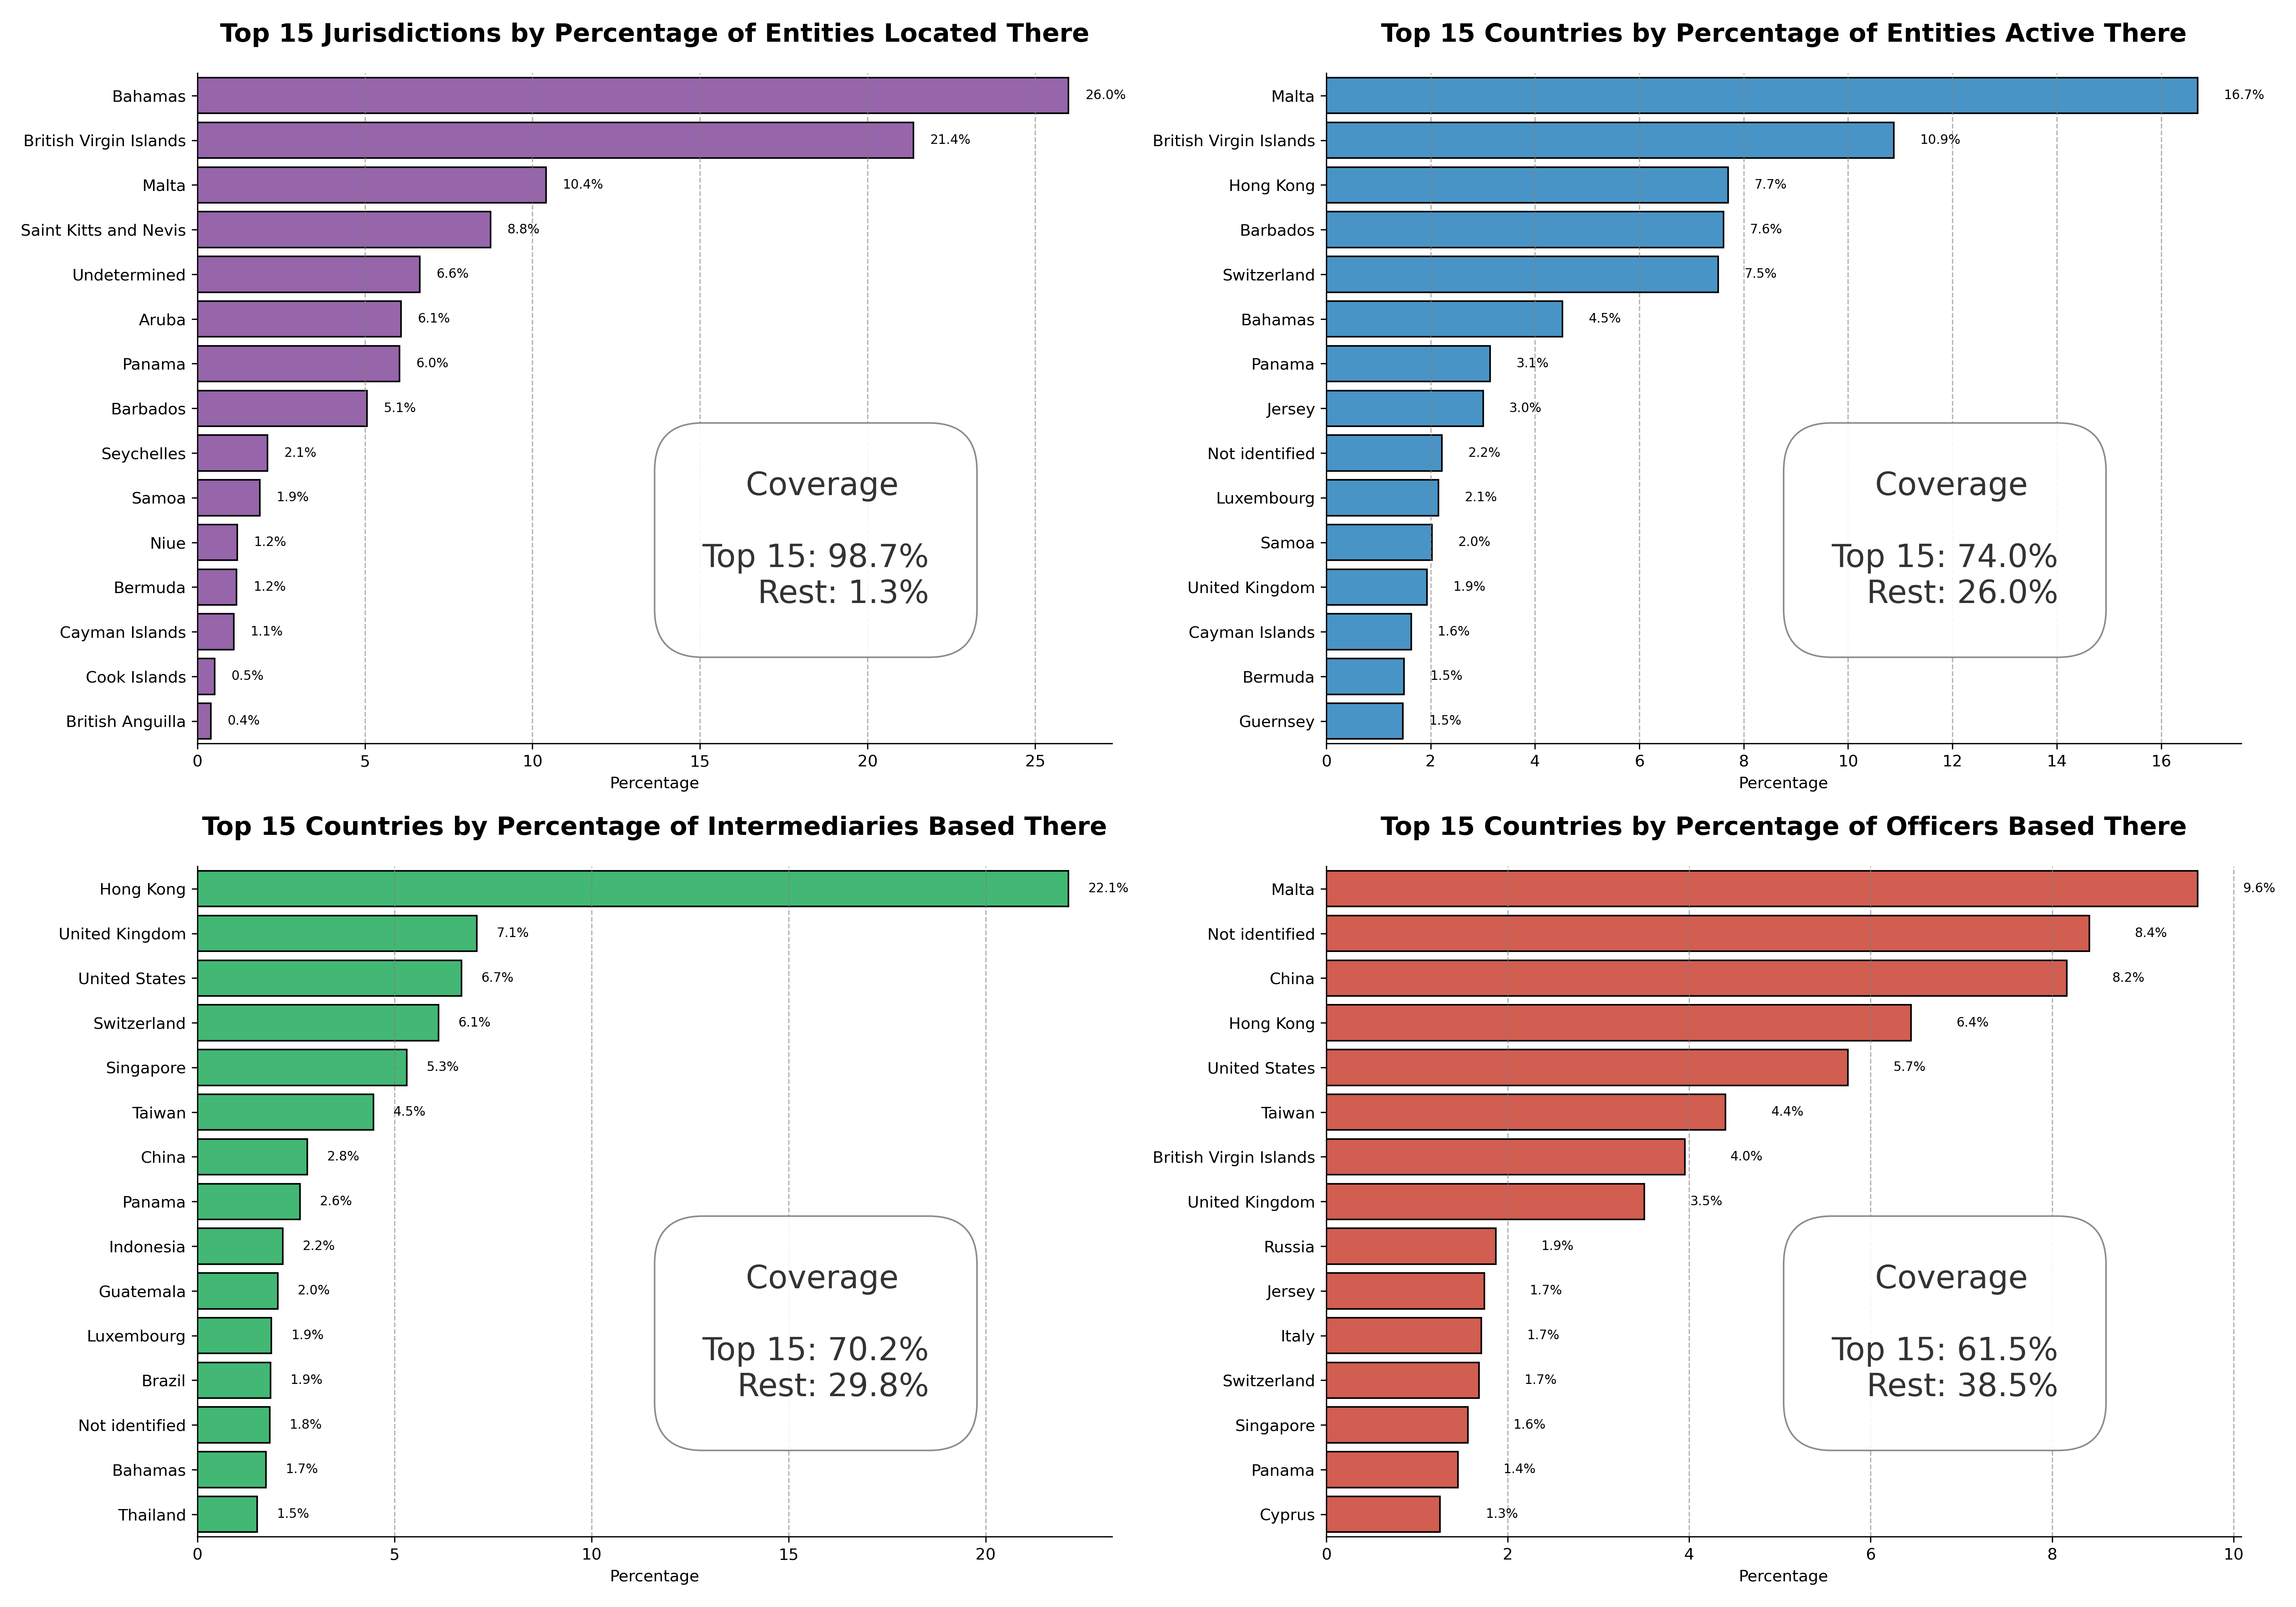
\includegraphics[width=0.9\textwidth]{Preliminary_Geography_Overview.png} % Increased width slightly for better readability if needed
    \caption{Geographical Concentration of Entities, Intermediaries, and Officers. Bar charts illustrate the percentage of total entities incorporated in the top 15 jurisdictions, entities with activity linked to the top 15 countries, intermediaries based in the top 15 countries, and officers associated with the top 15 countries.}
    \label{fig:preliminary_geography_overview}
\end{figure}

\subsubsection{Degree Distribution of Intermediaries}
\label{subsubsec:degree_dist_intermediaries}
A recurring theme, and one that underpins much of the analytical framework of this thesis, is the prevalence of power-law-like distributions in network metrics. This is particularly evident in the degree distribution of intermediaries, as illustrated in Figure \ref{fig:preliminary_powerlaw_fit}. The degree of an intermediary, in this context, represents the number of distinct entities they are connected to, serving as a proxy for their client load or market reach.

The observed distribution indicates that a small number of intermediaries are connected to a very large number of entities, forming "super-hubs" of activity, while the vast majority of intermediaries have relatively few connections. This characteristic aligns with findings from structural studies of similar datasets, such as Kejriwal and Dang's (2020) analysis of the Panama Papers, which also identified power-law degree distributions. Such a distribution suggests a highly heterogeneous system where certain intermediaries play a disproportionately significant role.

To formally assess this, the fit of the power-law model is compared to that of a log-normal distribution for the intermediary degree data. This comparison yielded a log-likelihood ratio $R = 57.0287$ with a $p$-value $< 0.0001$ (detailed in Section \ref{sec:3_3_analytical_methodologies} and implemented as per Clauset et al., 2009). This result strongly suggests that a power-law model provides a statistically significantly better fit than a log-normal model, or at the very least, indicates that the distribution is distinctly heavy-tailed. The implications of this scale-free or heavy-tailed characteristic are profound: it points towards a system where a few key intermediaries may act as critical "enablers" or "chokepoints" (Chang et al., 2023b; Christensen, 2024).

\begin{figure}[htbp]
    \centering
    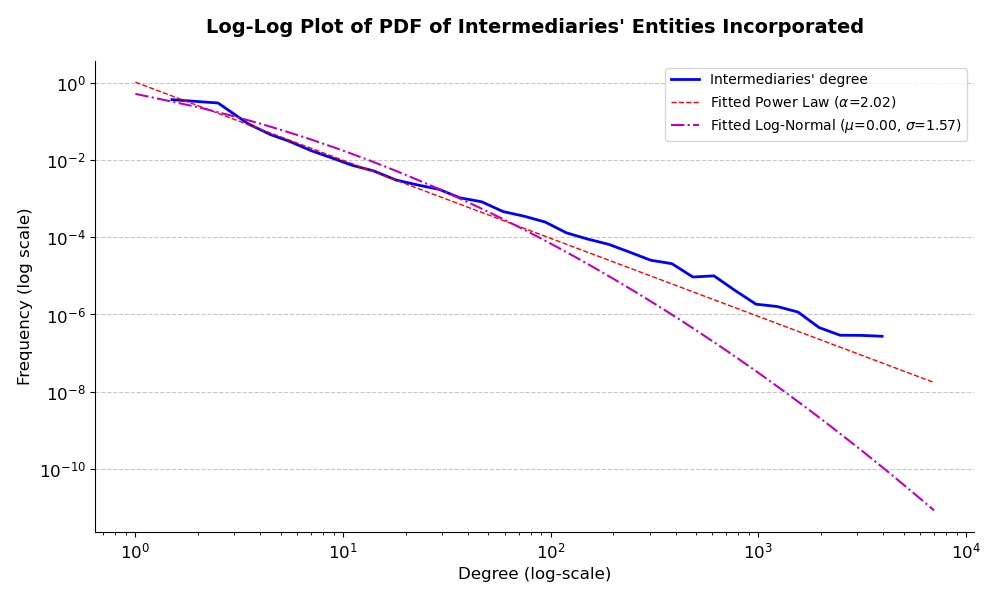
\includegraphics[width=0.8\textwidth]{Preliminary_Powerlaw_Fit.png}
    \caption{Degree Distribution of Intermediaries and Model Fits. The plot shows the probability density function (PDF) of intermediary degrees on a log-log scale. The empirical data (blue line) is compared against a fitted power-law distribution (red dashed line, $\alpha \approx 2.08$) and a fitted log-normal distribution (purple dash-dot line).}
    \label{fig:preliminary_powerlaw_fit}
\end{figure}


\section{Geographical Specialisation}
\label{sec:geographical_specialisation}

This section delves into the geographical patterns exhibited by intermediaries, focusing on the locations of their clients and the jurisdictions they select for entity incorporation. It covers specialization at both the country level of intermediary operation and through network analysis of co-service patterns across entities and jurisdictions.

\subsubsection{Intermediary Specialisation at the Country Level}
\label{subsubsec:intermediary_specialisation_country}

To understand how intermediaries based in specific countries tailor their services, we examine their client footprints and their preferred jurisdictions for incorporation. Heatmaps visually represent these patterns for intermediaries based in the top 15 countries by intermediary count: Hong Kong (HKG), Great Britain (GBR), the United States (USA), Switzerland (CHE), Singapore (SGP), Taiwan (TWN), China (CHN), Panama (PAN), Indonesia (IDN), Guatemala (GTM), Luxembourg (LUX), Brazil (BRA), Bahamas (BHS), Jersey (JEY), and Thailand (THA). Figures \ref{fig:geography_country_heatmaps_top5}, \ref{fig:geography_country_heatmaps_top6_10}, and \ref{fig:geography_country_heatmaps_top11_15} display these heatmaps, detailing the top client countries (by entity activity) and top incorporation jurisdictions for intermediaries in these key operational hubs. These visualizations generally indicate that intermediaries often serve a significant proportion of clients from their own country of operation, while their choice of incorporation jurisdictions tends to be far more outwardly focused and diverse.

The heatmaps reveal distinct national profiles. For instance, intermediaries in major financial centers like Hong Kong and Great Britain show relatively broad international client bases and utilize a range of offshore jurisdictions.

\begin{figure}[htbp]
    \centering
    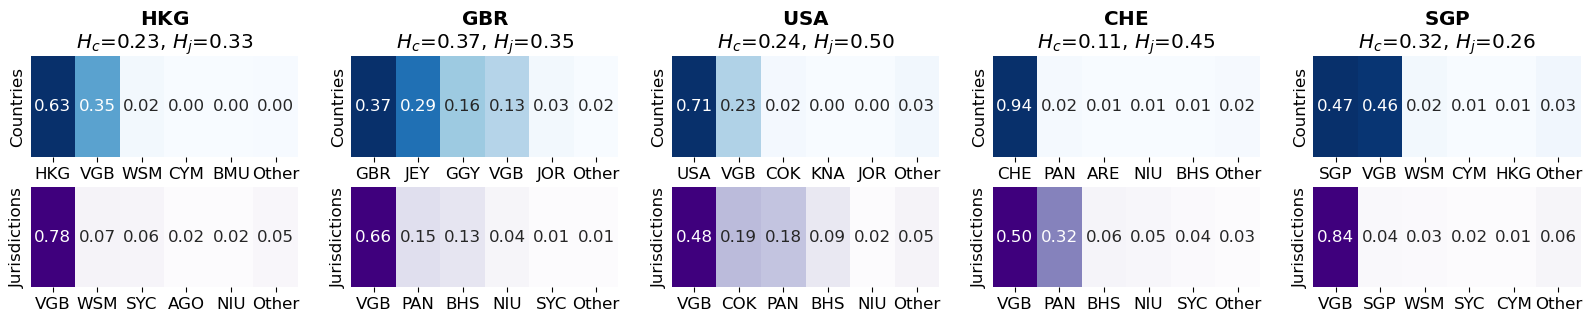
\includegraphics[width=0.9\textwidth]{Geography_Country_Heatmaps_Top5.png} % Adjusted width for potential better fit
    \caption{}
    \label{fig:geography_country_heatmaps_top5}
\end{figure}
\begin{figure}[htbp]
    \centering
    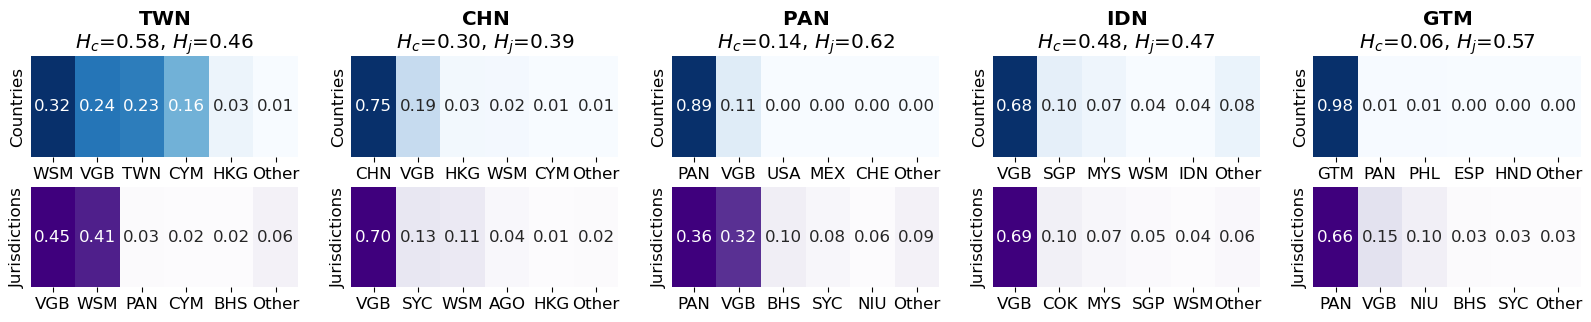
\includegraphics[width=0.9\textwidth]{Geography_Country_Heatmaps_Top6_10.png} % Adjusted width
    \caption{Client and Incorporation Jurisdiction Heatmap for Intermediaries in Top 6-10 Countries (TWN, CHN, PAN, IDN, GTM). Panels follow the same format as Figure \ref{fig:geography_country_heatmaps_top5}.}
    \label{fig:geography_country_heatmaps_top6_10}
\end{figure}

\begin{figure}[htbp]
    \centering
    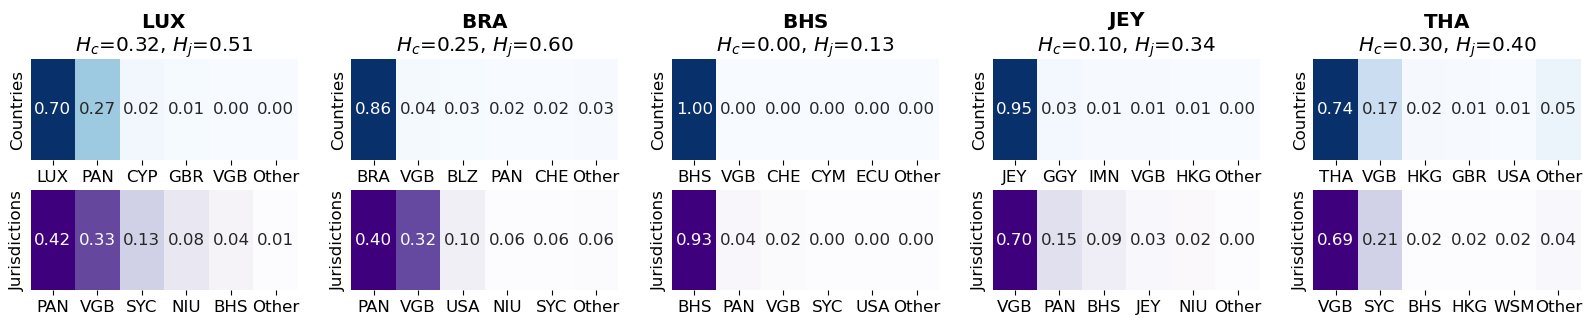
\includegraphics[width=0.9\textwidth]{Geography_Country_Heatmaps_Top11_15.png} % Adjusted width
    \caption{Each panel shows the distribution of client entity countries and incorporation jurisdictions for intermediaries based in the specified country. $H_c$ denotes country entropy and $H_j$ denotes jurisdiction entropy for that group of intermediaries.}
    \label{fig:geography_country_heatmaps_top11_15}
\end{figure}

A general trend observed is that intermediaries tend to be more diversified in their choice of \textit{incorporation jurisdictions} for their clients' entities compared to the geographical spread of the \textit{countries where their clients' entities are primarily active}. This is quantified by comparing the normalized entropy of jurisdictions used for incorporation ($H_j$) with the normalized entropy of client entity countries ($H_c$) at the aggregate level for intermediaries within each country. As shown in Figure \ref{fig:geography_country_level_entropy_distribution}, the distribution of jurisdiction entropy (mean = 0.48) is significantly higher than that of client country entropy (mean = 0.23). A two-sample Kolmogorov-Smirnov test confirms that these two distributions are statistically different (KS test: $p \approx 3 \times 10^{-7}$), suggesting that while client bases may be geographically somewhat concentrated, intermediaries draw upon a wider palette of offshore jurisdictions to structure entities. This aligns with the notion that intermediaries strategically select from a global "market for tax havens" (Laffitte, 2024) to meet diverse client needs, whereas client acquisition might be more localized.

\begin{figure}[htbp]
    \centering
    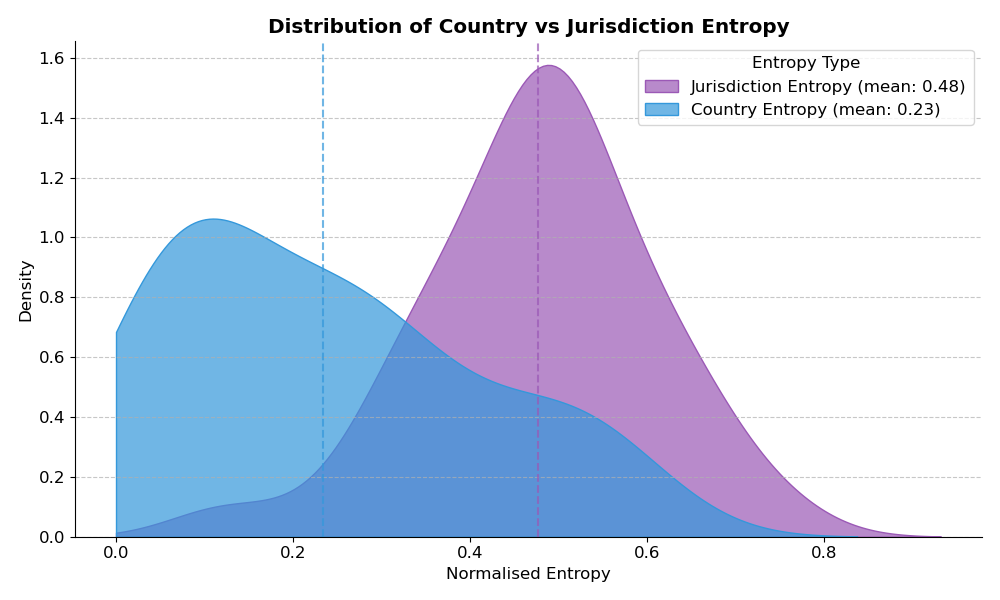
\includegraphics[width=0.8\textwidth]{Geography_Country_Level_Entropy_Distribution.png}
    \caption{Distribution of Normalized Entropy for Client Countries vs. Incorporation Jurisdictions, Aggregated at the Country Level of Intermediaries. The plot shows that intermediaries, when grouped by their country of operation, tend to use a more diverse set of incorporation jurisdictions ($H_j$, mean = 0.48) than the diversity observed in their clients' countries of activity ($H_c$, mean = 0.23).}
    \label{fig:geography_country_level_entropy_distribution}
\end{figure}

An illustrative example of specific geographical specialization is Cyprus (Figure \ref{fig:geography_country_heatmaps_cyprus}). Cyprus is well-documented in academic and policy literature for its strong financial links to Russia (e.g., Alstadsæter et al., 2022, note similar patterns for Dubai). While Russia is generally underrepresented in the broader ICIJ dataset, entities incorporated by Cypriot intermediaries show a significant Russian presence, with 12\% of such entities linked to Russia. This suggests a strong, specific association (a high "lift" in association analysis terms - though not formally tested here) for the Cyprus-Russia connection, as Russia appears minimally in the client portfolios of intermediaries from most other countries. The entropy values for Cyprus-based intermediaries ($H_c = 0.55, H_j = 0.53$) indicate moderate diversification in both client countries and incorporation jurisdictions.

\begin{figure}[htbp]
    \centering
    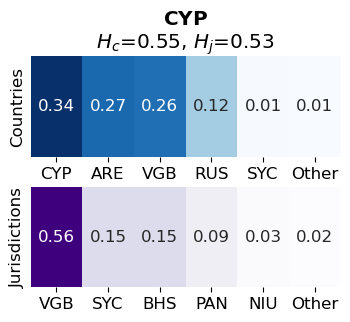
\includegraphics[width=0.8\textwidth]{Geography_Country_Heatmaps_Cyprus.png}
    \caption{Client and Incorporation Jurisdiction Heatmap for Cyprus-based Intermediaries ($H_c=0.55, H_j=0.53$). The heatmap shows that 12\% of entities serviced by Cypriot intermediaries have links to Russia; a notable concentration.}
    \label{fig:geography_country_heatmaps_cyprus}
\end{figure}

\subsubsection{Network of Countries Served by Intermediaries}
\label{subsubsec:network_countries_served}

While intermediaries operating at the country level exhibit specialization, particularly in their client bases, this section examines the specific clusters of countries served by individual intermediaries. At the individual intermediary level, clientele also tends to be highly concentrated in one or two countries, as shown by the distribution in Figure \ref{fig:geography_distribution_countries_by_intermediary}. This indicates that most intermediaries focus their client acquisition efforts narrowly. Interestingly, even as intermediaries grow larger (i.e., serve more entities, reflected by their degree), there is a very low correlation between the number of entities served and the number of distinct countries their clients' activities are linked to, suggesting that scaling often occurs through deeper penetration within existing client geographies rather than broad international expansion of the client base.

\begin{figure}[htbp]
    \centering
    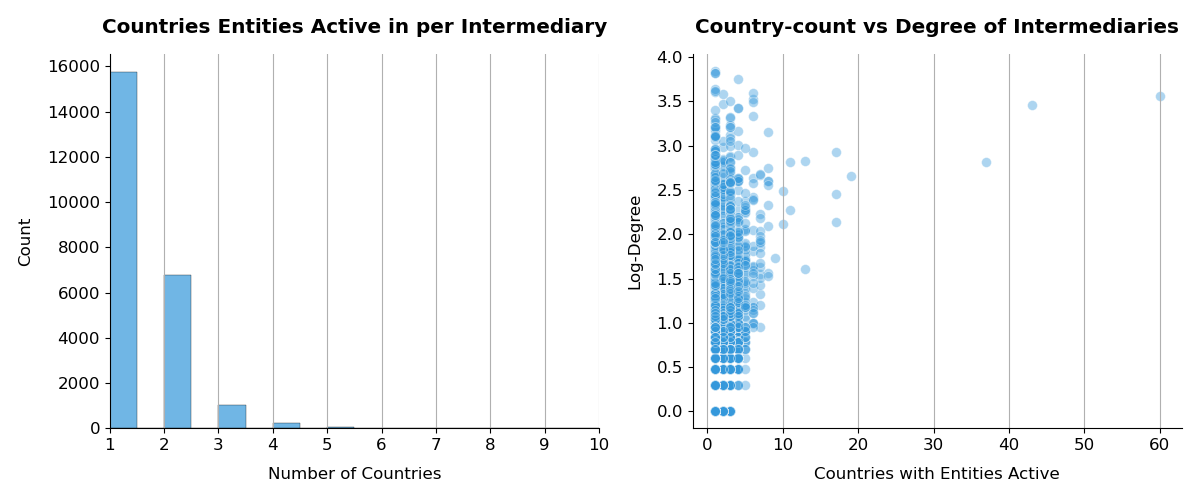
\includegraphics[width=0.8\textwidth]{Geography_Distribution_of_Countries_by_Intermediary.png}
    \caption{Distribution of the Number of Countries Linked to Entities Served per Intermediary. The distribution is heavily skewed, with most intermediaries serving entities linked to only one or a few countries - even high-degree intermediaries.}
    \label{fig:geography_distribution_countries_by_intermediary}
\end{figure}

To explore these co-service relationships further, a network of countries was constructed. In this network, countries are nodes, and an edge exists between two countries if at least one intermediary serves clients (entities) linked to both. The weight of the edge reflects the number of distinct intermediaries serving clients in both countries. The resulting full country network consists of 121 nodes (countries) and 2,716 edges. Key summary statistics for this network are presented in Table \ref{tab:country_network_summary}. 

\begin{table}[htbp]
\centering
\caption{Summary Statistics for the Full Country Co-Service Network}
\label{tab:country_network_summary}
\begin{tabular}{lc}
\toprule
\textbf{Metric}                        & \textbf{Value}    \\
\midrule
Number of Nodes               & 121      \\
Number of Edges               & 2716     \\
Network Density               & 0.3741   \\
Average Degree                & 44.89    \\
Average Clustering Coefficient & 0.7728   \\
\bottomrule
\end{tabular}
\end{table}

Visualising such dense graphs is incredibly challenging - and to be entirely honest, the rest of the thesis could be filled with differently filtered versions of this graph, illuminating some other aspect of it. Therefore, to identify the most important connections, the network was filtered using principles from association analysis. Edges are displayed only if they 1) meet a minimum support threshold (representing at least 0.008 of all intermediaries' country-pair connections, meaning the pair is co-serviced by at least that fraction of intermediaries who service multiple countries) and 2) a lift score of 1.5 or higher. Lift measures how much more frequently two countries are co-serviced than would be expected if their servicing by intermediaries were independent. This filtering ensures that the visualized connections are not only reasonably frequent but also represent associations significantly stronger than chance, that they are both common links as well as carrying statistical signal. The resulting filtered network, or "backbone," thus highlights the most robust and significant co-service relationships. While the exact number of nodes included is sensitive to the choice of the lift and support thresholds here, this "backbone" as I term it, is relatively stable across a range of thresholds.

The nodes in the network visualization (Figure \ref{fig:geography_cross_country_network}) are coloured in two ways: first, by communities identified using the Louvain modularity maximization algorithm (Blondel et al., 2008), which groups densely interconnected countries; and second, by regime type using VDem data, as described in Section \ref{sec:3_2}. This dual coloring was intended to explore whether regime type influences intermediary operations and co-service patterns, a factor suggested by literature on offshore secrecy strategies (e.g. Chang et al., 2023b).

\begin{figure}[htbp]
    \centering
    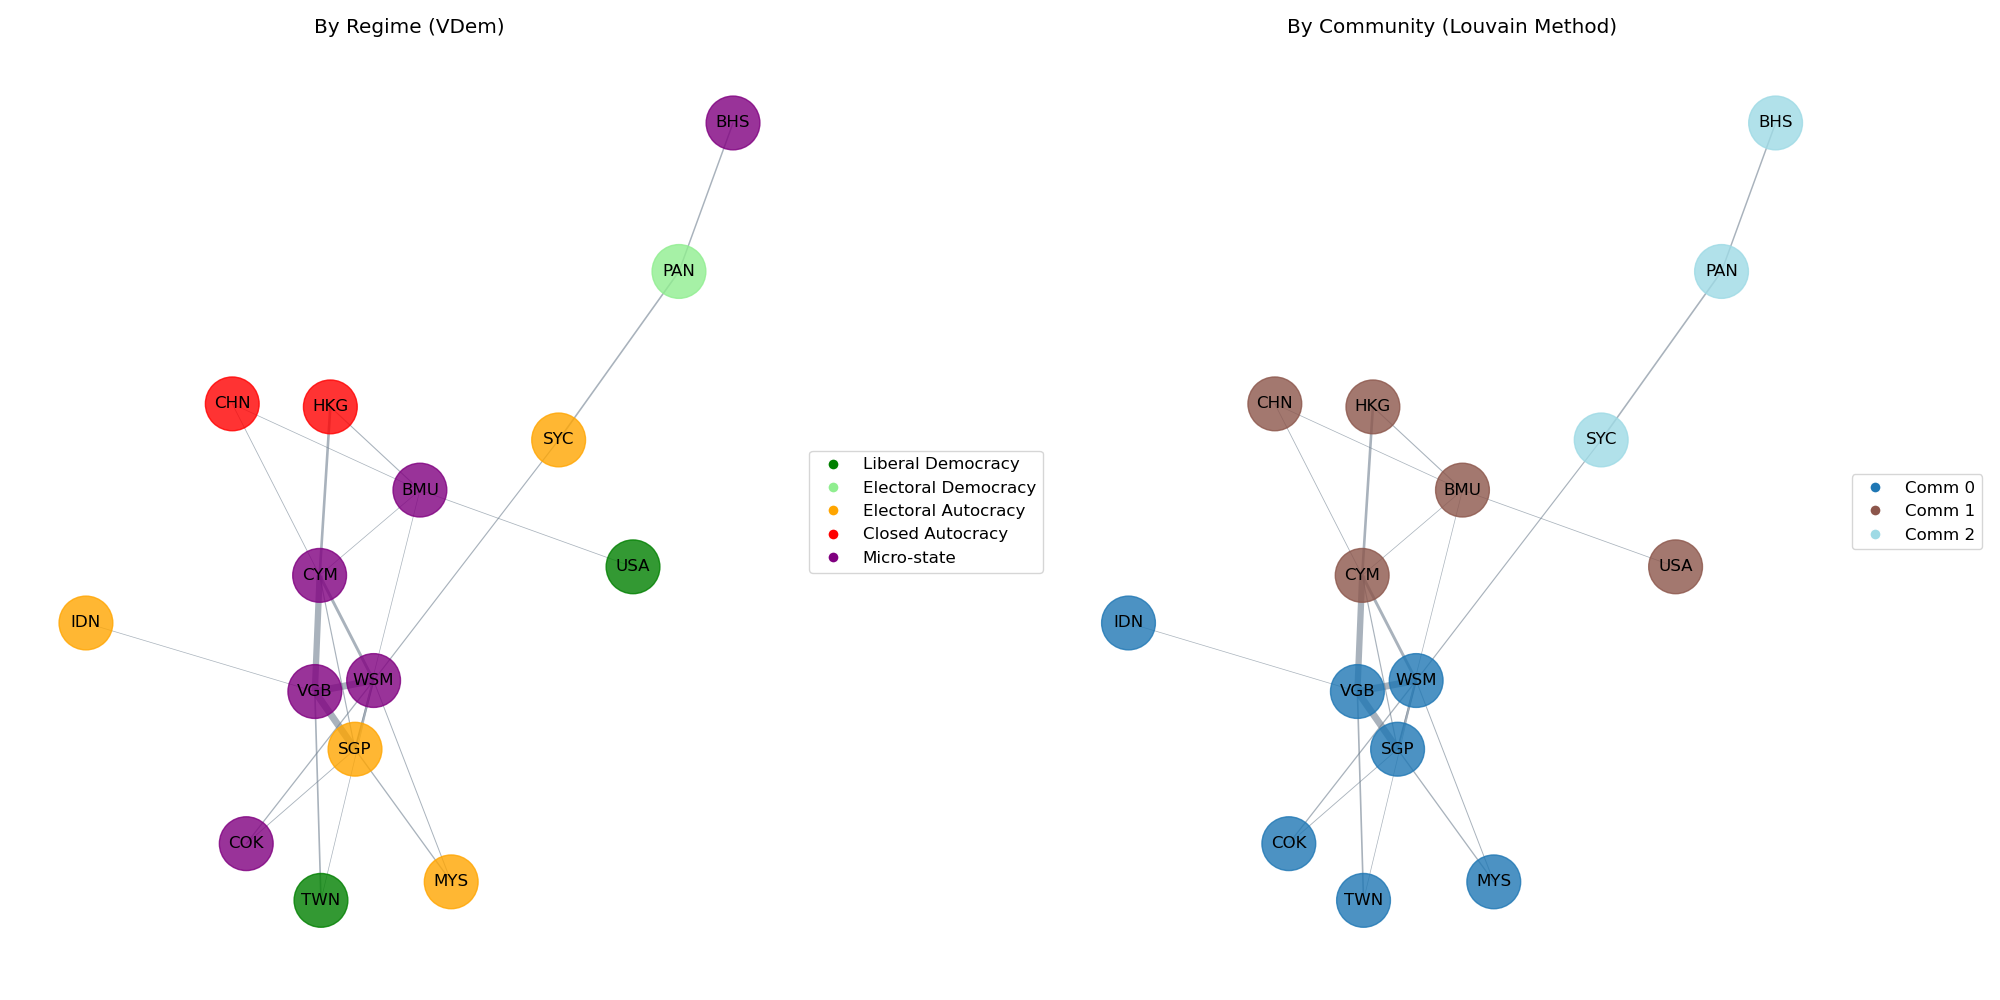
\includegraphics[width=0.9\textwidth]{Geography_Cross_Country_Network.png}
    \caption{Filtered Network of Co-Served Countries, Coloured by Louvain Community (left legend) and Regime Type (right legend). Edges shown have support $\ge 0.008$ and lift $\ge 1.5$. Node size can be proportional to degree or another centrality measure.}
    \label{fig:geography_cross_country_network}
\end{figure}

\paragraph{Interpretation of the Filtered Country Network Structure}
The filtered network (Figure \ref{fig:geography_cross_country_network}) reveals a sparse yet highly structured set of relationships, forming a distinct core-periphery structure. A central core of interconnected nodes is evident, particularly involving VGB (British Virgin Islands), CYM (Cayman Islands), and SGP (Singapore), along with their strong links to HKG (Hong Kong) and BMU (Bermuda).

When coloured by regime type, no clear large-scale clustering emerges that aligns strictly with political systems. The central cluster itself is diverse, including Micro-states (VGB, CYM, BMU), jurisdictions classified as Closed Autocracies (HKG, reflecting its unique status), and Electoral Autocracies (SGP). Liberal Democracies such as the USA and TWN (Taiwan) are present but connect to nodes of various different regime types. This visual evidence supports the notion that regime type, while potentially a factor in individual elite choices (Chang et al., 2023c), is not a primary driver of these strong, systemic co-service relationships at the country-network level. Economic roles, historical ties, and financial infrastructure likely play more dominant roles in shaping this backbone.

The Louvain community detection method, which is data-driven, reveals distinct groupings based on the density of co-service links:
\begin{itemize}
    \item \textbf{Community 0 (Dark Blue):} This is the largest community, featuring prominent offshore centers like VGB and CYM, major Asian economies/financial hubs like SGP, TWN (Taiwan), MYS (Malaysia), IDN (Indonesia), and Pacific jurisdictions like COK (Cook Islands) and likely WSM (Samoa, if present in the filtered graph). This highlights strong ties between several offshore financial centers and key Asian economies.
    \item \textbf{Community 1 (Brown):} This community comprises major economies like the USA and CHN (China), alongside HKG (Hong Kong) and the offshore jurisdiction BMU (Bermuda), indicating a distinct Atlantic-Pacific nexus involving Bermuda.
    \item \textbf{Community 2 (Light Blue):} A smaller, distinct community consisting of PAN (Panama), SYC (Seychelles), and BHS (Bahamas), all of which are significant offshore jurisdictions.
\end{itemize}
Most nodes in this backbone network are connected within two to three steps, indicating a relatively compact structure despite the filtering.

\paragraph{Centrality in the Country Network}
Centrality metrics calculated on the full 121-node co-service network (detailed in Appendix Tables \ref{tab:appendix_country_betweenness_app} and \ref{tab:appendix_country_eigenvector_app}) identify key players.
\textbf{VGB (British Virgin Islands)} is dominant, exhibiting the highest betweenness and eigenvector centrality, underscoring its pivotal role in connecting diverse client countries through shared intermediaries. The \textbf{USA} ranks second in both measures, reflecting its economic importance and the global reach of its client base serviced by international intermediaries. The USA is linked to BMU (Bermuda) in the filtered graph's Community 1. \textbf{HKG (Hong Kong) \& CHN (China)} also feature prominently in centrality scores and are central to Community 1. Numerous \textbf{Micro-states} (BMU, BHS, CYM) show high centrality, consistent with their specialized roles in offshore finance. \textbf{SGP (Singapore)} is another key, highly central node, bridging various parts of the network. In general, high centrality in the full network translates to a significant structural role in this filtered backbone, indicating that the most connected countries in the overall system also form the core of the strongest co-service relationships.

\paragraph{Significant Country Associations}
Lift scores from the association analysis (top associations detailed in Appendix Table \ref{tab:appendix_significant_country_associations_app}, filtered for co-occurrences $\ge 20$) reveal particularly strong and statistically significant pairings, many of which are visualized in Figure \ref{fig:geography_cross_country_network} (those with lift $\ge 1.5$).
Key findings include:
\begin{itemize}
    \item Strong \textbf{Micro-state synergies} are evident. For instance, the WSM-CYM (Samoa-Cayman Islands) pairing shows a high lift of 6.78, and VGB-CYM (British Virgin Islands-Cayman Islands) has a lift of 1.91. These indicate that intermediaries servicing clients in one of these micro-states are substantially more likely to also service clients in the other, suggesting complementary service offerings or established pathways for specific client types. The CYM-BMU (Cayman Islands-Bermuda) link is exceptionally strong with a lift of 13.5.
    \item A critical \textbf{China-Bermuda nexus} emerges with CHN-BMU showing a very high lift of 15.3. This suggests Bermuda acts as a particularly favored intermediary hub for clients linked to China. This is complemented by the USA-BMU link (lift 4.92), highlighting Bermuda's role in Community 1 of the filtered network, connecting major economic powers.
    \item Robust \textbf{Asian connections} are underscored by pairs like SGP-MYS (Singapore-Malaysia, lift 5.27). Singapore (SGP) also shows strong co-service patterns with various Micro-states such as WSM (Samoa, lift 3.04) and CYM (Cayman Islands, lift 3.89), reinforcing its role as a key hub in Community 0.
    \item A distinct \textbf{PAN-SYC-BHS nexus} (Community 2) is confirmed with pairings like PAN-SYC (Panama-Seychelles) having a lift of 3.89.
    \item Crucially, high lift values are common \textbf{across different regime types}. For example, China (Closed Autocracy) has a very high lift with Bermuda (Micro-state), and the USA (Liberal Democracy) also has a significant lift with Bermuda. This reinforces the earlier observation that factors beyond regime similarity, such as specialized financial services, established legal and commercial pathways, or historical ties, are potent drivers of these strong co-service relationships.
\end{itemize}

\subsubsection{Network of Jurisdictions Used by Intermediaries}
\label{subsubsec:network_jurisdictions_used}

Shifting focus from client locations to incorporation locations, this section analyzes the network of jurisdictions that intermediaries use in combination. The full jurisdiction co-usage network, where an edge exists if an intermediary incorporates entities in both jurisdictions (weighted by the number of such intermediaries), comprises 41 nodes and 347 edges. Summary statistics are provided in Table \ref{tab:jurisdiction_network_summary}. The distribution of the number of distinct jurisdictions used per intermediary is shown in Figure \ref{fig:geography_distribution_jurisdictions_by_intermediary}, indicating that most intermediaries utilize a small portfolio of jurisdictions, though some use many.

\begin{table}[htbp]
\centering
\caption{Summary Statistics for the Full Jurisdiction Co-Usage Network}
\label{tab:jurisdiction_network_summary}
\begin{tabular}{lc}
\toprule
\textbf{Metric}                        & \textbf{Value}    \\
\midrule
Number of Nodes               & 41       \\
Number of Edges               & 347      \\
Network Density               & 0.4232   \\
Average Degree                & 16.93    \\
Average Clustering Coefficient & 0.8155   \\
\bottomrule
\end{tabular}
\end{table}

\begin{figure}[htbp]
    \centering
    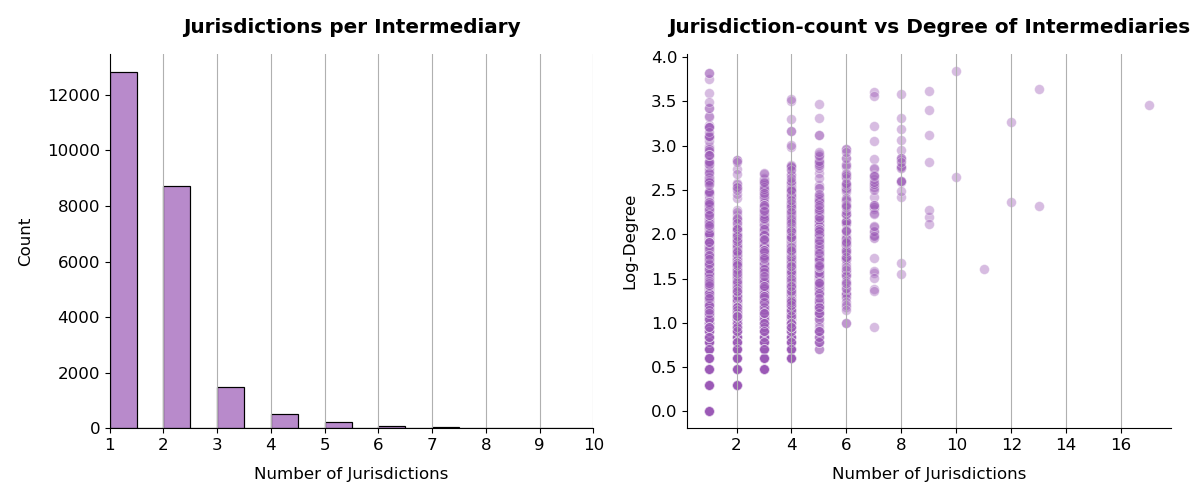
\includegraphics[width=0.8\textwidth]{Geography_Distribution_of_Jurisdictions_by_Intermediary.png}
    \caption{Distribution of the Number of Distinct Jurisdictions Used per Intermediary. Most intermediaries use only one or two jurisdictions for incorporation, but a tail of intermediaries uses a broader portfolio.}
    \label{fig:geography_distribution_jurisdictions_by_intermediary}
\end{figure}

Figure \ref{fig:geography_cross_jurisdiction_network} presents a filtered "backbone" of these co-usage patterns, applying the same support ($\ge 0.008$) and lift ($\ge 1.5$) thresholds as for the country co-service network. Nodes are coloured by their predominant legal technology profile (derived from Laffitte, 2024, as detailed in Section \ref{sec:3_2}) and by Louvain communities. The image displays the most prominent nodes in this filtered network, including CRI (Costa Rica), SGP (Singapore), CYP (Cyprus), GBR (Great Britain), BLZ (Belize), AGO (Angola), HKG (Hong Kong), CYM (Cayman Islands), COK (Cook Islands), MYS (Malaysia), BHS (Bahamas), SYC (Seychelles), PAN (Panama), NIU (Niue), WSM (Samoa), and USA.

\begin{figure}[htbp]
    \centering
    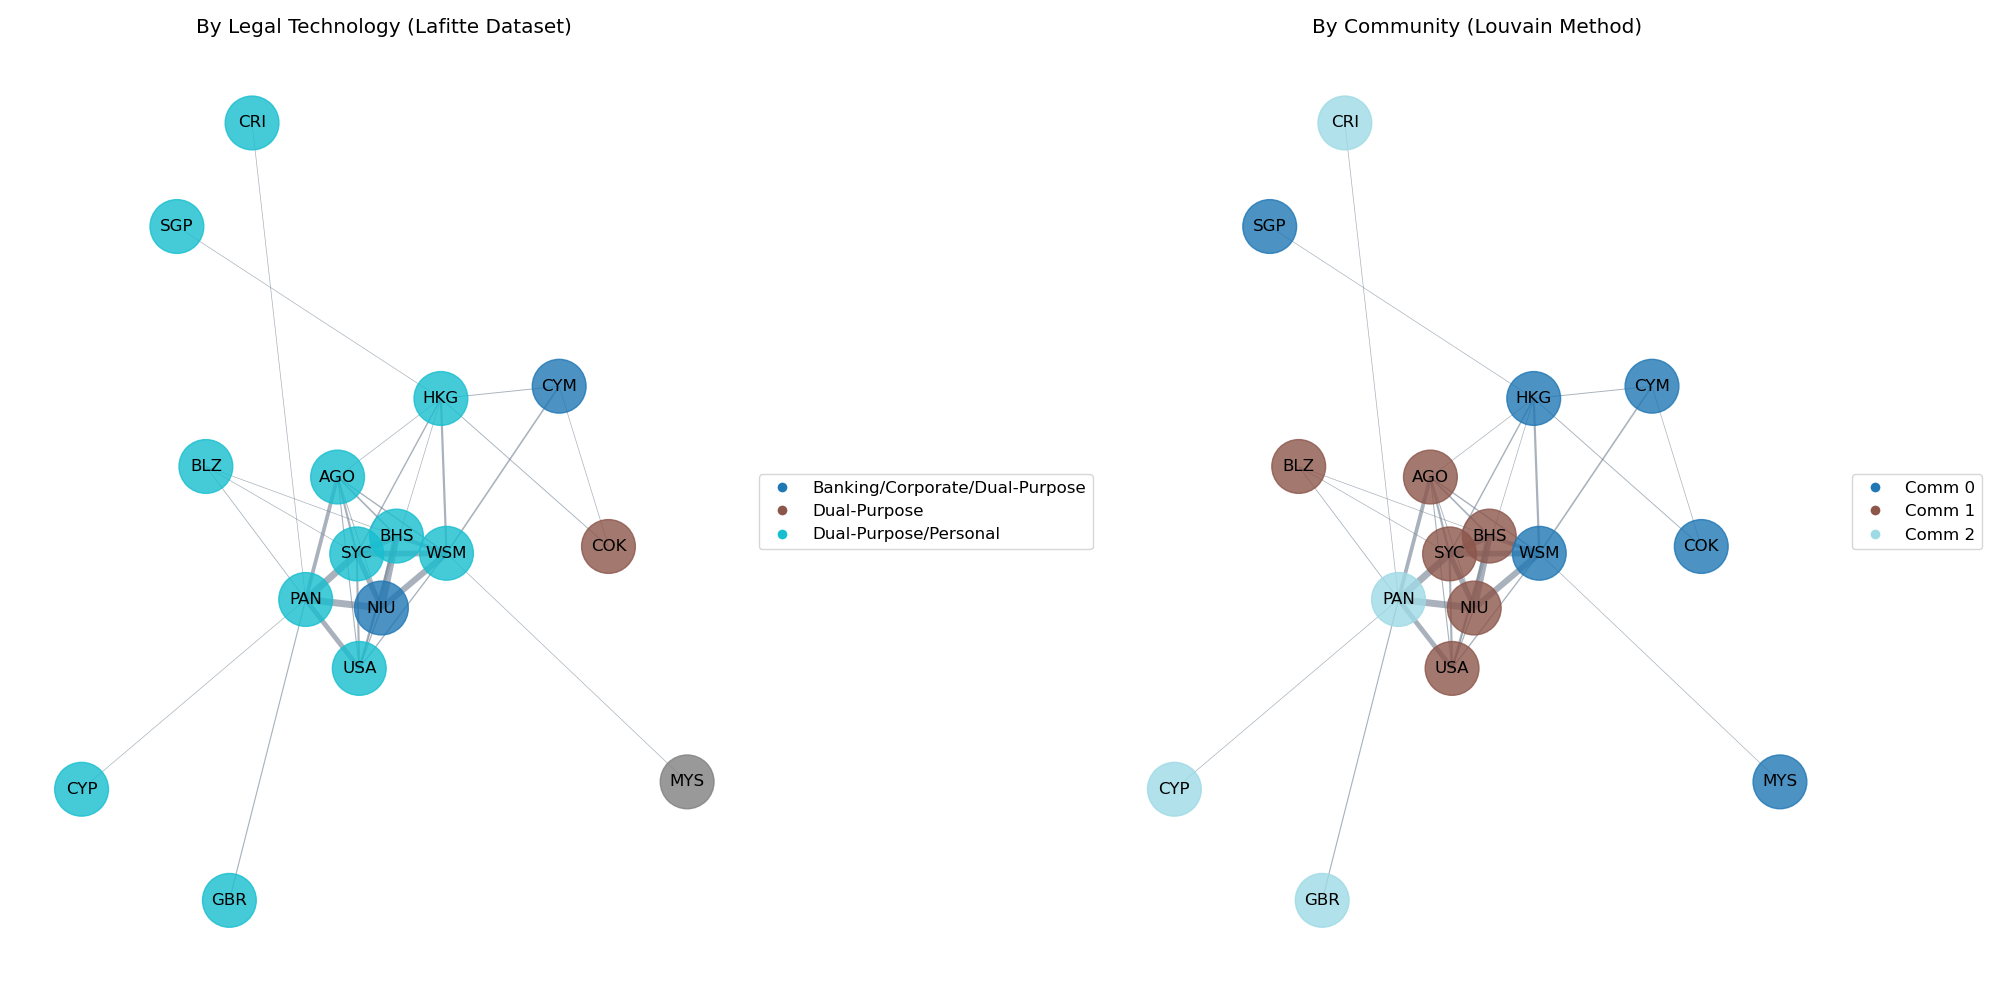
\includegraphics[width=0.9\textwidth]{Geography_Cross_Jurisdiction_Network.png}
    \caption{Filtered Network of Co-Used Jurisdictions, Coloured by Predominant Legal Technology (left legend) and Louvain Community (right legend). Edges shown have support $\ge 0.008$ and lift $\ge 1.5$.}
    \label{fig:geography_cross_jurisdiction_network}
\end{figure}

\paragraph{Interpretation of the Filtered Jurisdiction Network Structure}
The filtered jurisdiction network (Figure \ref{fig:geography_cross_jurisdiction_network}) reveals a central, densely connected core. Key jurisdictions in this core include BHS (Bahamas), SYC (Seychelles), AGO (Angola), WSM (Samoa), NIU (Niue), PAN (Panama), USA, and HKG (Hong Kong).

When coloured by their predominant legal technology profile (Laffitte, 2024), the central cluster is overwhelmingly dominated by jurisdictions offering \textbf{"Dual-Purpose"} legal technologies (e.g., International Business Companies - IBCs). This strongly supports the observation that central jurisdictions in this co-usage network are those providing flexible, widely applicable corporate vehicles suitable for both corporate and personal wealth structuring. 

Louvain community detection identifies the following groupings based on co-usage patterns:
\begin{itemize}
    \item \textbf{Community 1 (Brown):} This is the largest and most central community, encompassing jurisdictions like USA, PAN, NIU, BHS, SYC, AGO, and WSM. These are largely characterized by "Dual-Purpose" legal technologies.
    \item \textbf{Community 0 (Dark Blue):} This community includes HKG, CYM (Cayman Islands), and COK (Cook Islands), combining jurisdictions known for "Banking/Corporate/Dual-Purpose" (like HKG) with those strong in "Dual-Purpose/Personal" (like CYM, COK).
    \item \textbf{Community 2 (Light Blue):} This community is more peripheral in the filtered network and includes SGP (Singapore), CRI (Costa Rica), CYP (Cyprus), GBR (Great Britain), BLZ (Belize), and MYS (Malaysia), representing a mix of financial centers and specialized offshore jurisdictions.
\end{itemize}

\paragraph{Centrality in the Jurisdiction Network}
Centrality metrics for the full 41-jurisdiction co-usage network (detailed in Appendix Tables \ref{tab:appendix_jurisdiction_betweenness_app} and \ref{tab:appendix_jurisdiction_eigenvector_app}) are revealing.
\textbf{VGB (British Virgin Islands)} ranks first in both betweenness and eigenvector centrality in the full network, confirming its paramount importance as an incorporation jurisdiction. However, it is strikingly absent from the filtered graph in Figure \ref{fig:geography_cross_jurisdiction_network}. This implies that while VGB is co-used with many other jurisdictions by numerous intermediaries, these individual pairings might not meet the specific high support and lift thresholds chosen for this backbone view (requiring at least 20 co-occurrences and lift $\ge 1.5$). This suggests VGB's role might be more as a general-purpose, widely connected jurisdiction whose strong pairings are numerous but perhaps more diffuse, rather than concentrated in extremely high-lift niche combinations that also meet the co-occurrence threshold.
\textbf{BHS (Bahamas)} and \textbf{PAN (Panama)} rank second and third, respectively, in overall centrality and are visibly central within the filtered graph, particularly in Community 1. \textbf{HKG (Hong Kong)} and \textbf{CYM (Cayman Islands)} are also highly central in the full network and form a core part of Community 0 in the filtered view. Most other top-ranked jurisdictions by centrality align with their prominence in the backbone, with VGB being the main exception due to the filtering criteria.

\paragraph{Significant Jurisdiction Associations}
Association analysis, focusing on lift scores from statistically significant pairs with at least 20 co-occurrences (detailed in Appendix Table \ref{tab:appendix_significant_jurisdiction_associations_app}), highlights robust co-usage patterns:
\begin{itemize}
    \item The dominant \textbf{Community 1 (largely "Dual-Purpose" hubs)} shows very high mutual lift values. For instance, BHS-NIU (Bahamas-Niue) has a lift of 4.6 (support 0.016), and NIU-WSM (Niue-Samoa) has a lift of 5.3 (support 0.012). NIU (Niue) appears as a critical connector within this cluster of Pacific and Caribbean jurisdictions, also showing strong lift with SYC (Seychelles, lift 4.1, support 0.010).
    \item \textbf{Community 0 (financial centers and specialized OFCs)}: The HKG-CYM (Hong Kong-Cayman Islands) pairing shows a strong lift of 5.8 (support 0.0018), indicating a significant tendency for intermediaries using one to also use the other. WSM-CYM (Samoa-Cayman Islands) also shows a notable lift of 4.6 (support 0.0031).
    \item Strong co-usage is observed between jurisdictions offering \textbf{similar legal technology profiles}. For example, many of the high-lift pairs within Community 1 involve jurisdictions predominantly offering "Dual-Purpose" or "Dual-Purpose/Personal" technologies.
\end{itemize}


\section{Functional Specialisation of Intermediaries}
\label{sec:functional_specialisation}

This section transitions from the geographical patterns of intermediary activity to an exploration of their functional roles. Drawing upon the typology developed by the EU (2017) (De Groen, 2017), which distinguishes between roles such as Tax Expert, Legal Expert, Administrator, and Investment Advisor, we investigate whether these classifications correspond to distinct operational characteristics. A central theme is the differentiation between intermediaries primarily offering \textit{personalised advice} versus those focused on \textit{aid in incorporation} and ongoing entity management.

The analysis in this section primarily utilizes a classified random sample of intermediaries. This approach is adopted because, as will be shown, intermediaries with the highest degrees (i.e., those connected to the largest number of entities) are not representative of the broader intermediary population in terms of functional type (see Figure \ref{fig:specialisation_classification_distribution}). The detailed filtering process for this enriched random sample, ensuring high-confidence classifications, is illustrated in Figure \ref{fig:appendix_filtering_enrichment} (and further detailed in Appendix \ref{sec:appendix_enrichment_filtering_details} if you have such an appendix section).

\begin{figure}[htbp]
    \centering
    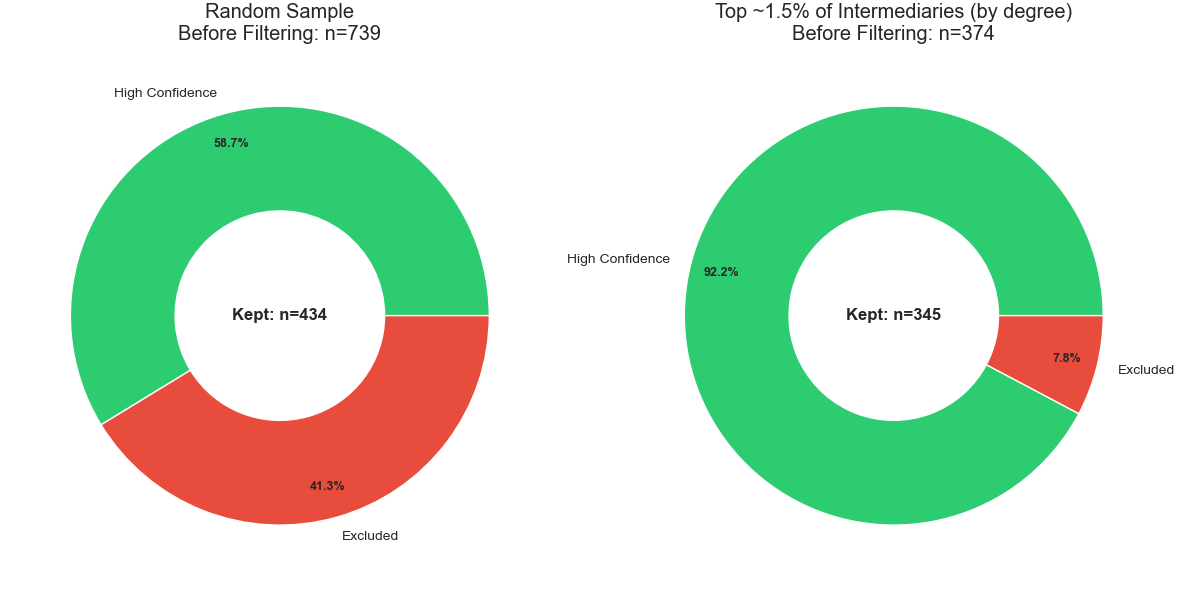
\includegraphics[width=0.8\textwidth]{Appendix_Filtering_of_Enrichment.png}
    \caption{Filtering Process of the Enriched Random Sample for Functional Classification. This flowchart illustrates the steps taken to arrive at the final set of intermediaries with high-confidence functional classifications used in this section's analysis.}
    \label{fig:appendix_filtering_enrichment}
\end{figure}

\subsubsection{Different Levels of Connectivity: Personalised Advice vs. Aid in Incorporation}
\label{subsubsec:connectivity_functional}

A key differentiator among intermediary types is expected to be their scale of operation, proxied by their degree (the number of entities they are connected to). Intermediaries providing bespoke, personalised advice (e.g., Tax Experts, Investment Advisors) might typically serve fewer clients than those offering more standardized services like entity incorporation and administration (e.g., Administrators, and some Legal Experts specializing in volume).

Figure \ref{fig:specialisation_cdf_degrees} presents the Cumulative Distribution Function (CDF) of degrees for each intermediary classification within the random sample. Visual inspection suggests differences in these distributions, particularly between groups like Tax Experts and Administrators.

\begin{figure}[htbp]
    \centering
    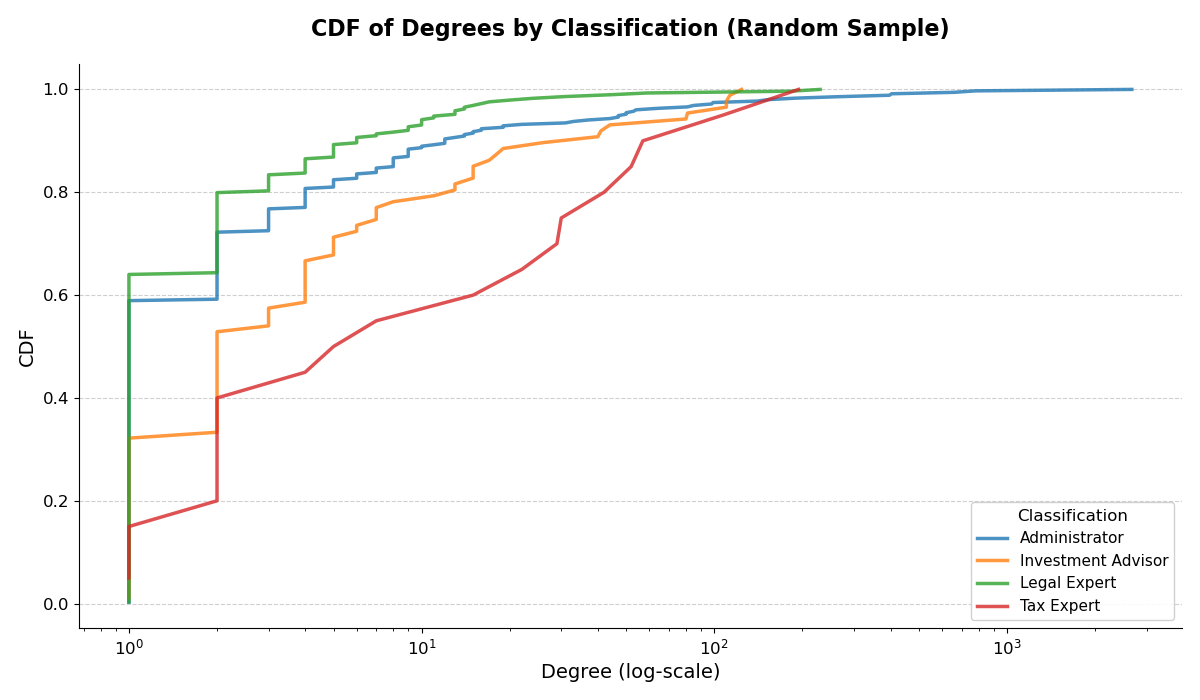
\includegraphics[width=0.8\textwidth]{Specialisation_CDF_of_Degrees_by_Classification_Random_Sample.png}
    \caption{Cumulative Distribution Function (CDF) of Degrees by Intermediary Classification (Random Sample). The plot shows distinct degree profiles, with Tax Experts and Investment Advisors generally having lower degrees than Administrators and Legal Experts.}
    \label{fig:specialisation_cdf_degrees}
\end{figure}

To formally test these observations, a Kruskal-Wallis H test was performed, which indicated a statistically significant difference in degree distributions among the four classifications (H(3) = 51.243, $p < 0.0001$). Subsequent pairwise two-sample Kolmogorov-Smirnov (KS) tests, with Bonferroni correction for the six unique pairs (corrected $\alpha = 0.05/6 \approx 0.0083$), were conducted to pinpoint specific differences:
\begin{itemize}
    \item \textbf{Administrator vs. Investment Advisor:} Significant difference (KS = 0.267, $p_{corr} \approx 0.0024$).
    \item \textbf{Administrator vs. Legal Expert:} No significant difference (KS = 0.077, $p_{corr} = 1.0000$).
    \item \textbf{Administrator vs. Tax Expert:} Significant difference (KS = 0.439, $p_{corr} \approx 0.0282$).
    \item \textbf{Investment Advisor vs. Legal Expert:} Significant difference (KS = 0.318, $p_{corr} < 0.0001$).
    \item \textbf{Investment Advisor vs. Tax Expert:} No significant difference (KS = 0.285, $p_{corr} = 1.0000$). % Original p was 0.6899, Bonferroni makes it 1.0
    \item \textbf{Legal Expert vs. Tax Expert:} Significant difference (KS = 0.490, $p_{corr} \approx 0.0042$).
\end{itemize}
These results support the notion of two broader functional groups based on connectivity. The "personalised advice" types (Tax Experts and Investment Advisors) do not significantly differ from each other in degree distribution. Similarly, the "aid in incorporation/management" types (Legal Experts and Administrators) do not significantly differ from each other. However, comparisons across these broader groups (e.g., Tax Expert vs. Legal Expert, Investment Advisor vs. Administrator) reveal significant differences, with the personalised advice types generally having lower degrees.

This distinction is further highlighted when comparing the composition of the random sample with a sample of the top approximately 1.5\% of intermediaries by degree (Figure \ref{fig:specialisation_classification_distribution}). The top-degree sample is overwhelmingly composed of Administrators, who constitute a much smaller fraction of the random sample. Conversely, the random sample shows a higher prevalence of Legal Experts, Investment Advisors, and Tax Experts, who are less dominant among the highest-degree intermediaries. This underscores that intermediaries specializing in high-volume entity administration are distinct from those providing more individualized services.

\begin{figure}[htbp]
    \centering
    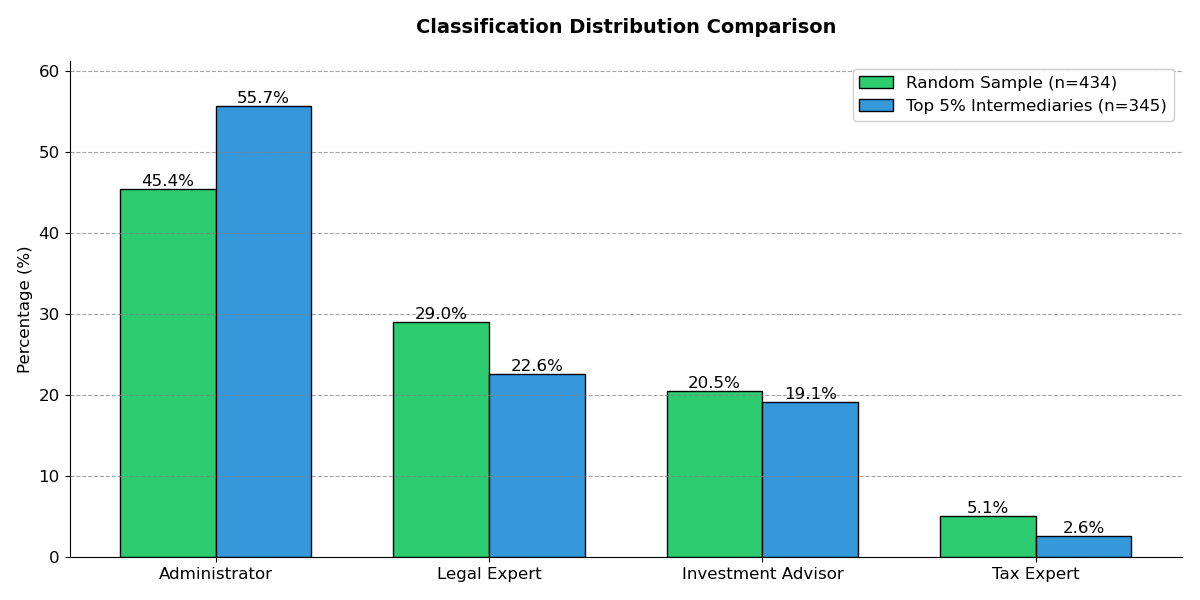
\includegraphics[width=0.8\textwidth]{Specialisation_Classification_Distribution_Comparison.png}
    \caption{Distribution of Intermediary Classifications: Random Sample vs. Top $\approx$1.5\% by Degree. The random sample shows a more diverse mix of functional types, while the top-degree sample is heavily dominated by Administrators.}
    \label{fig:specialisation_classification_distribution}
\end{figure}

\subsubsection{Different Activities: Instruments and Service Offerings}
\label{subsubsec:activities_functional}

Beyond connectivity, we examine if intermediary types differ in their operational activities, using five key metrics:
\begin{enumerate}
    \item \textbf{Jurisdiction Entropy}: Diversity in the jurisdictions where they incorporate entities.
    \item \textbf{Client Country Entropy}: Diversity in the countries their clients' entities are linked to.
    \item \textbf{Regime Entropy}: Diversity in the political regimes of the countries where client entities are linked.
    \item \textbf{Legal Technology Entropy}: Diversity in the types of legal technologies (Laffitte, 2024) prevalent in the jurisdictions they use for incorporation.
    \item \textbf{Bearer Instrument Usage}: A binary indicator of whether the intermediary has serviced entities using bearer instruments.
\end{enumerate}

Figure \ref{fig:specialisation_average_entropy_bearer} displays the average values of these metrics for each intermediary classification in the random sample. Pairwise comparisons using Mann-Whitney U tests for entropy measures and Fisher's exact test for bearer instrument usage were conducted, with a Bonferroni correction applied for the 30 comparisons (5 metrics $\times$ 6 pairs, corrected $\alpha = 0.05/30 \approx 0.00167$).

\begin{figure}[htbp]
    \centering
    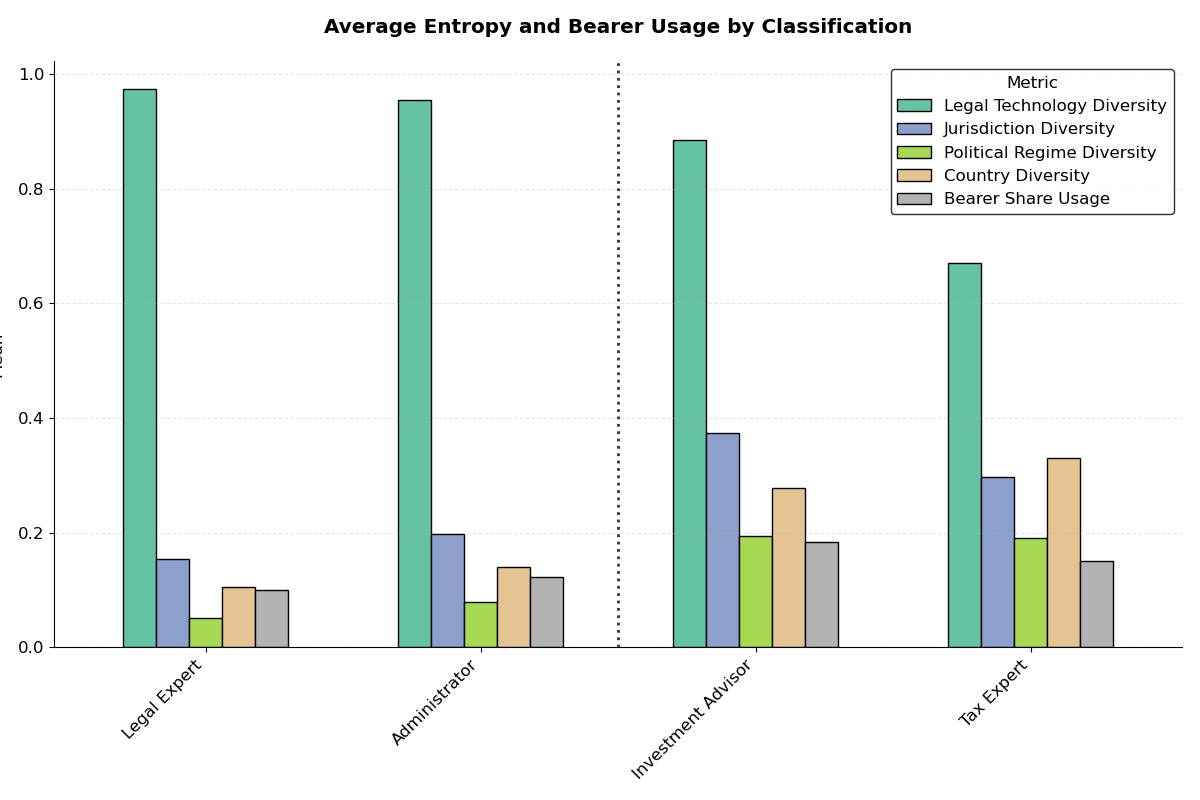
\includegraphics[width=0.8\textwidth]{Specialisation_Average_Entropy_and_Bearer_Usage_by_Classification.png}
    \caption{Average Entropy Measures and Bearer Instrument Usage by Intermediary Classification (Random Sample). Error bars could represent standard errors if available.}
    \label{fig:specialisation_average_entropy_bearer}
\end{figure}

The statistical tests revealed several significant differences (detailed results in Appendix \ref{sec:appendix_functional_specialisation_stats} if you have one, otherwise summarize key findings):

\textbf{Legal Technology Entropy:}
Legal Experts exhibit significantly higher diversity in the legal technologies of the jurisdictions they use compared to Investment Advisors ($U = 15330.5, p_{corr} < 0.0001$) and Tax Experts ($U = 4560.5, p_{corr} < 0.0001$). Administrators also show significantly higher diversity than Investment Advisors ($U = 17801.5, p_{corr} \approx 0.0047$) and Tax Experts ($U = 5401.5, p_{corr} < 0.0001$). This suggests that Legal Experts and Administrators engage with a broader array of jurisdictional legal frameworks. No significant difference was found between Legal Experts and Administrators, nor between Investment Advisors and Tax Experts.

\textbf{Jurisdiction Entropy:}
Legal Experts show significantly higher diversity in incorporation jurisdictions compared to Investment Advisors ($U = 9271.0, p_{corr} < 0.0001$). Similarly, Administrators demonstrate greater jurisdiction diversity than Investment Advisors ($U = 12187.5, p_{corr} \approx 0.0012$). Other pairwise comparisons for jurisdiction entropy did not yield statistically significant differences after Bonferroni correction. This indicates that Legal Experts and Administrators tend to utilize a wider range of jurisdictions than Investment Advisors.

\textbf{Regime Entropy:}
Legal Experts exhibit significantly higher diversity in the political regimes of their client countries compared to Investment Advisors ($U = 10185.0, p_{corr} < 0.0001$) and Tax Experts ($U = 2100.5, p_{corr} \approx 0.0001$). Administrators also show significantly higher regime diversity than Investment Advisors ($U = 13170.5, p_{corr} \approx 0.0044$). This pattern suggests that Legal Experts and Administrators may cater to clienteles originating from a more diverse set of political environments.

\textbf{Client Country Entropy:}
Legal Experts demonstrate significantly higher diversity in their client countries compared to Investment Advisors ($U = 10164.5, p_{corr} \approx 0.0001$) and Tax Experts ($U = 1863.5, p_{corr} < 0.0001$). Administrators also have significantly more diverse client countries than Tax Experts ($U = 2462.0, p_{corr} \approx 0.0057$). This implies that Legal Experts, and to some extent Administrators, engage with clients from a broader range of countries.

\textbf{Bearer Instrument Usage:}
After Bonferroni correction, \textbf{no statistically significant differences} were found in the propensity to use bearer instruments among any of the intermediary classifications. This suggests that, within this classified random sample, the use of these high-anonymity instruments is not strongly associated with a particular functional type of intermediary.

In summary, Legal Experts and Administrators tend to exhibit greater diversity across various geographical and legal-technical dimensions of their service offerings compared to Tax Experts and Investment Advisors. This aligns with the notion that the former group, often involved in broader incorporation and management services, may engage with a wider array of jurisdictional options and client origins. The "personalised advice" groups (Tax Experts and Investment Advisors) appear more focused in these respects. The lack of differentiation in bearer instrument usage is a notable finding, suggesting other factors may drive their deployment.

